\section{\textsc{Vinaigrette}}

\subsection*{Zutaten für 100ml:}

\begin{tabular}{p{7.5cm} p{7.5cm}}
	& \\
	25ml Essig & Salz, Pfeffer \& Zucker \\
	75ml Öl & 
\end{tabular}

\subsection*{Serviervorschlag:}

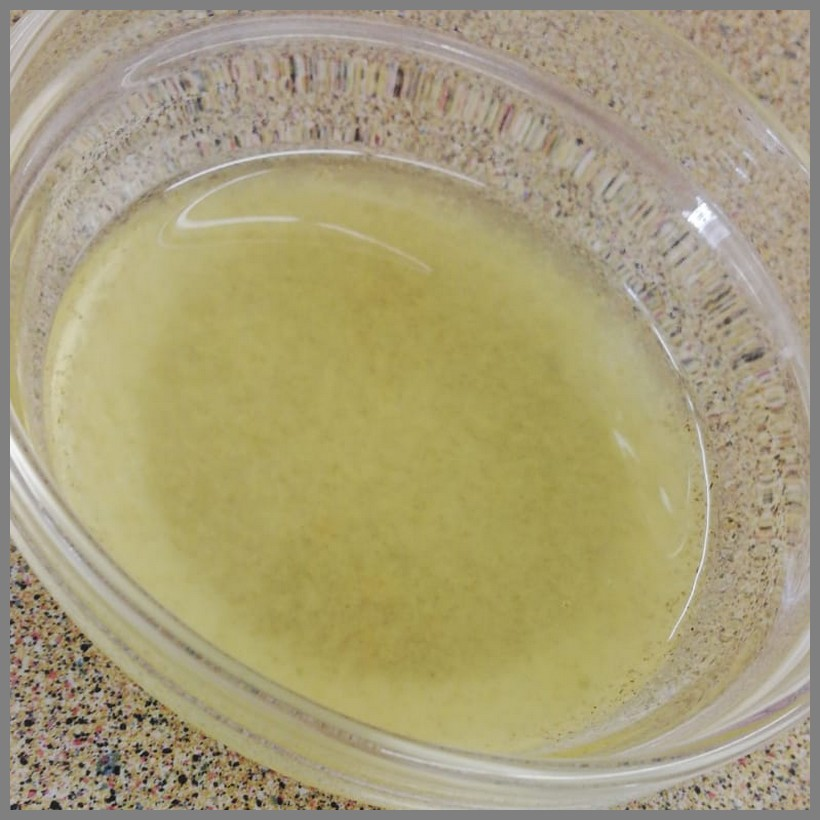
\includegraphics[width=\textwidth]{img/d_vinaigrette.jpeg} \cite{vinaigrette}

\subsection*{So geht's:}

\begin{tabular}{p{15cm}}
	\\
	Salz in Essig auflösen, Öl dazurühren.\\
	Das Ganze mit wenig Pfeffer würzen und anschliessend mit Zucker abrunden.\\
	\textbf{Tipp:} Der Essig kann durch Zitronen- oder Limettensaft ersetzt werden.\\
	\\
	Geeignet zu allen Salaten.
\end{tabular}
